\documentclass[a4papaer,12pt]{article}

\usepackage[left=25mm, top=20mm, right=25mm, bottom=30mm,nohead,nofoot]{geometry}
\usepackage[T2A]{fontenc}
\usepackage[utf8]{inputenc}
\usepackage[english,russian]{babel}
\usepackage[compatibility=false]{caption}
\usepackage{subcaption}
\usepackage{wrapfig}
\usepackage{graphics, graphicx}
\graphicspath{{./images/}}
\setcounter{tocdepth}{4}
\usepackage{hyperref}
\hypersetup{unicode=true}
\usepackage{amssymb,latexsym} 
\usepackage{MnSymbol}
\usepackage{mathrsfs}
\usepackage[nottoc,numbib]{tocbibind}
\usepackage{float}
\usepackage{listings}
\usepackage{multirow}
\usepackage{hhline}
\usepackage{delarray}
\usepackage{color,colortbl}
\usepackage{float}

\renewcommand{\listoffigures}{\begingroup  % add number to list of graphics
\tocsection
\tocfile{\listfigurename}{lof}
\endgroup}
\renewcommand{\listoftables}{\begingroup  % add number to list of tables
\tocsection
\tocfile{\listtablename}{lot}
\endgroup}

\begin{document}
\begin{titlepage}
	\center
		Санкт-Петербургский Политехнический
		университет \\ Петра Великого\\
		Институт прикладной математики и механики
		\\ \textbf{Высшая школа прикладной математики и вычислительной физики}

	\vfill ~
	\textbf{
		\\ \large Отчёт
	}
    \\ о летней производственной практике 

	\vfill ~

    \begin{flushleft}
    \underline{Выполнил:}  \hspace{\fill} студент гр.3640102/00201 \textbf{Лансков Н.В.} \linebreak[2]
	\underline{Руководитель:} \hspace{\fill} \textbf{Савчук Д.А.} \\
    \end{flushleft}

\vfill

{\large}	Санкт-Петербург
\\ 2021
\end{titlepage}

\tableofcontents
\newpage

\section{Введение}
В ходе летней практики я работал в компании ITS\cite{its}. Я решал много различных задач для разных проектов. Также 
в ходе практики я получил опыт управления командами разработчиков, общения с заказчиками и планирования проектов.
Это был интересный управленческий опыт, однако в рамках данного отчёта я опишу только технические задачи, 
которые были решены мной в рамках практики.

\section{Цели и задачи}

\begin{itemize}
    \item Добавить возможность динамически устанавливать метатеги для вебстраниц.
    \item Реализовать сервер для приложения, позволяющего получить от специалистов консультацию по вопросам трудоустройства.
    \item Оптимизировать процесс сборки нового приложения с нуля до полностью работоспособного состояния.
\end{itemize}

\section{Описание проделанной работы}

\subsection{Шаблонизация openresty}

В экосистеме современных веб приложений обычно участвует веб сервер.
В нашей компании мы используем в качестве веб сервера nginx.
Nginx раздаёт клиентам по запросу статические файлы или перенаправляет
поступивший запрос соответствующему приложению на нашем сервере.
И иногда перед возвратом пользователю запрошенной html страницы требуется
выполнить какие-то дополнительные действия. В частности, у нас появилась
необходимость снабжать страницу, которая отправляется клиенту, определёнными метатегами,
которые специфичны для каждой страницы. Чтобы автоматизировать данную задачу,
мы используем openresty\cite{openresty}. Это такая технология, которая позволяет выполнять код на
языке lua непосредственно при обработке nginx-ом запроса.
Если в обычной конфигурации nginx для раздачи статических файлов используется директива
\textbf{try\_files}, то с openresty мы заменяем один \textbf{location} блок на три:
в первом у нас обычная директива \textbf{try\_files}, если мы находим нужный файл
- отдаём его, если нет - переходим во второй \textbf{location} блок, в котором нгинкс
просто выполняет код скрипта на lua. И после этого мы переходим в последний блок-обработчик,
который уже отдаёт запрошенный файл, который был сгенерирован скриптом \cite{openresty_habr}.
На данный момент при помощи lua выполняются следующие обработки веб-страниц:

\begin{enumerate}
    \item Получение данных по апи и заполнение метатегов
    \item Предобработка текста в формате html - фильтрация html тегов
\end{enumerate}

\begin{figure}[H]
    \begin{subfigure}[b]{.49\linewidth}
    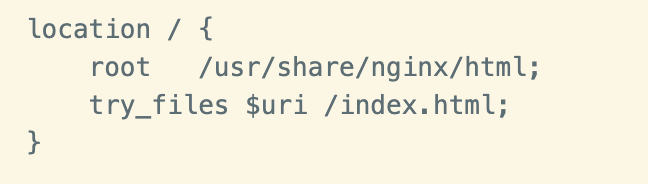
\includegraphics[width=\linewidth]{1}
    \caption{Обычная конфигурация блока обработки запросов}
    \end{subfigure}
    \begin{subfigure}[b]{.49\linewidth}
    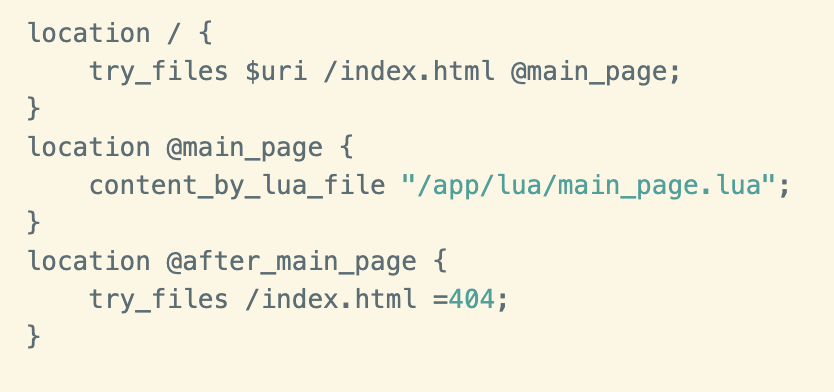
\includegraphics[width=\linewidth]{2}
    \caption{Пример конфигурации с использованием openresty}
    \end{subfigure}
\end{figure}

\subsection{Автоматизация деплоя при помощи docker-compose и bash}

В ходе практики также была усовершенствована система сборки готовых прилоджений и их 
запуска. При не очень большой инфраструктуре проще всего использовать такие инструменты
как docker-compose и bash скрипты. В ходе практики была произведена реорганизация 
конфигураций, позволяющая свести вывод приложения в рабочее состояние запуском одного скрипта.

\subsection{CRUD бэкенд для приложения поиска работы}

За июнь нашей кампанией был разработан проект, позволяющий тем, кто испытывает трудности при поиске работы
получить профессиональную консультацию у HR специалистов. Мной была разработана схема базы данных 
и реализовано приложение\cite{cvtr_api_docs} на python с использованием фреймворка flask\cite{flask}.  

\begin{figure}[H]
    \centering
    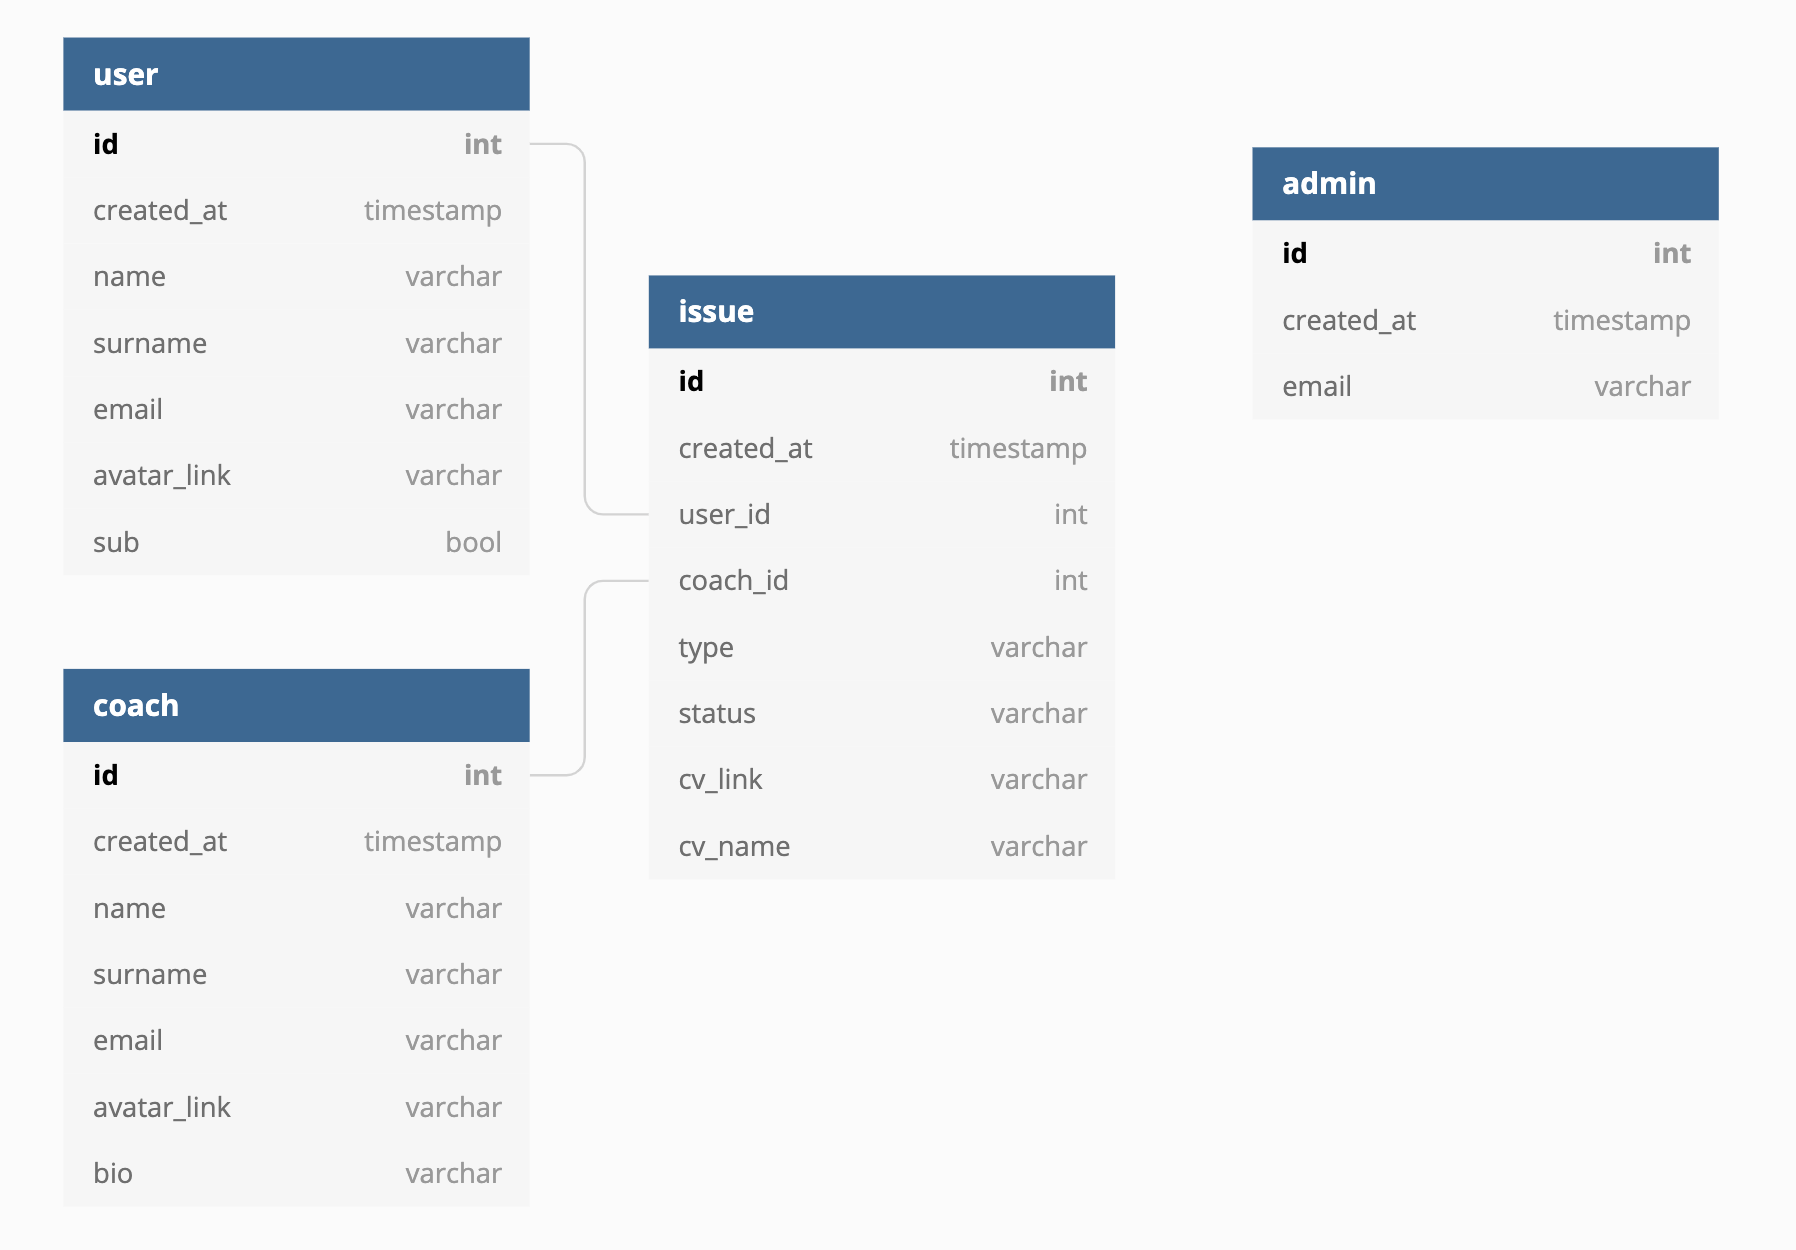
\includegraphics[width=0.7\linewidth]{3}
    \caption{Схема базы данных сервера}
\end{figure}

\newpage
\bibliographystyle{unsrt}
\bibliography{references}

\end{document}

